% !TeX root = ./Lsfem.tex
\documentclass[11pt,a5paper,notitlepage]{article}
\usepackage{amsmath}							            % American Mathematical Society package.
\usepackage{amsfonts}
\usepackage{amssymb}
\usepackage[english]{babel}
\usepackage{bm}									         % Bold math.
\usepackage[utf8]{inputenc}
\usepackage[T1]{fontenc}
\usepackage[style=german]{csquotes}
\usepackage{graphicx}							         % Define font colors, page colors, boxes with background color, rotate text in a box, scale text vertically and horizontally, put graphics in a box.
\usepackage{verbatim}							         % Multiline comments.
\usepackage{setspace}							         % Adjust line spacing.
\usepackage{parskip}
\setlength{\parindent}{0pt}
\usepackage{fancyhdr}							         % Fancy headers.
\linespread{1}
\usepackage[font=normalsize]{caption}  		 	   % Captions for figures inside minipages. Allows setting alignment inside captions.
\usepackage{subcaption}
\usepackage[retainorgcmds]{IEEEtrantools}  		   % Best tool for multiline equations or equation arrays.
\usepackage[unicode]{hyperref} 					      % Hyperlinks ToC entries to their respective pages.
\hypersetup{
    colorlinks,
    citecolor=black,
    filecolor=black,
    linkcolor=black,
    urlcolor=black }
\usepackage{url} 								            % Allows long URLs.
\usepackage{placeins} 							         % FloatBarrier.
\usepackage{booktabs}							         % TabItem (manually insert list item dot).
\usepackage{xcolor}								         % Required by tabu.
\usepackage{colortbl}							         % Required by tabu.
\usepackage{tabu}								            % Width-adjustable tabular.
\usepackage{multirow}							         % Columns spanning multiple rows.
\newcommand{\tabitem}{~~\llap{\textbullet}~~}	   % TabItem command.
\usepackage{wrapfig}							            % Figures which text can flow around.
\usepackage{physics}                               % For braket notation.
\usepackage{icomma}                                % Intelligent comma for decimal separators.
\usepackage{longtable}                             % For tabulars that split across pages.
\usepackage{listings}                              % For beautiful code.


% Math Symbol Abbreviations
\def\rcurs{{\mbox{$\resizebox{.09in}{.08in}{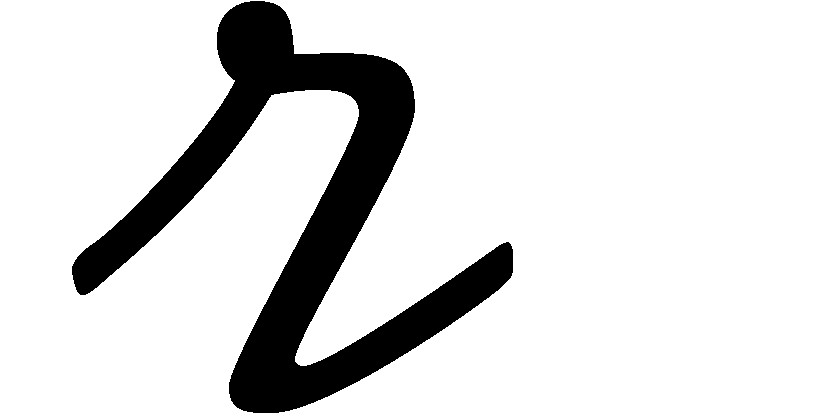
\includegraphics[trim= 1em 0 14em 0,clip]{TeX/ScriptR}}$}}}		% Cursive r.
\def\brcurs{{\mbox{$\resizebox{.09in}{.08in}{
\includegraphics[trim= 1em 0 14em 0,clip]{TeX/BoldR}}$}}}		% Bold cursive r.
\renewcommand{\arraystretch}{1.3} 				                        % List line spacing.
\newcommand{\ud}{\mathrm{d}} 					                           % Differential operator.
\newcommand{\uD}{\mathrm{D}}					                           % Capital D differential operator.
\newcommand{\pd}{\partial}						                           % Partial differential operator.
\newcommand{\del}{\bm{\nabla}}					                        % Bold nabla.
\newcommand{\mathbsf}[1] {\bm{\mathsf{#1}}}
\newcommand{\textbsf}[1] {\textbf{\textsf{#1}}}
\renewcommand{\Re}{\operatorname{Re}}		  	                        % Real-part-of-complex-number operator.
\renewcommand{\Im}{\operatorname{Im}} 			                        % Imaginary-part-of-complex-number operator.


% Paragraph-to-Equation Spacing
\setlength{\belowdisplayskip}{0pt} 			% Razmik pod enačbo, ko je vrstica polna.
\setlength{\abovedisplayskip}{0pt} 			% Razmik nad enačbo, ko je vrstica polna.
\setlength{\belowdisplayshortskip}{0pt}  		% Razmik pod enačbo, ko vrstica ni polna.
\setlength{\abovedisplayshortskip}{0pt}   		% Razmik nad enačbo, ko vrstica ni polna.

\pagestyle{fancy}	% Setting for FancyHdr package. Must occur before length adjustments.

% FIRST PAGE LAYOUT / VERTICAL LENGTHS
\setlength{\voffset}{-1.2in}					% Top to Header Top Margin = 1 inch+\voffset
\setlength{\topmargin}{8mm}					% Header Top Margin Height
\setlength{\headheight}{1.75cm}
\setlength{\headsep}{0.35cm}					% Header Lower Margin Height
\setlength{\textheight}{174mm}					% Header Lower Margin to Footer height
\setlength{\footskip}{7mm}
% FIRST PAGE LAYOUT / HORIZONTAL LENGTHS
\setlength{\headwidth}{132mm}
\setlength{\hoffset}{-1.0in}					% Left page padding = 1 inch + \hoffset
\setlength{\oddsidemargin}{8mm}
\setlength{\textwidth}{132mm}
\setlength{\marginparsep}{0.0cm}
\setlength{\marginparwidth}{0.0cm}				% Width of "side notes margin."

\fancyhead[L]{Marko Petek \\[0.3cm] }
\fancyhead[C]{
\includegraphics[height=1.6cm]{Slike/logo-um-fnm}}
\fancyhead[R]{Maribor,\\ 13.\ VII.\ 2019 \\[0.15cm] }
\cfoot{\thepage}								      % Footer center = page number.			
\renewcommand{\headrulewidth}{0.0cm}			% Horizontal line in header. 0 = no horizontal line.
\renewcommand{\footrulewidth}{0.0cm}			% Horizontal line in footer

\begin{document}
   \begin{center}
      \textbf{\LARGE{Block Structured Mesh}}\\[0.25cm]
   \end{center}

\section*{BlockMesh.cs}
   Two 2nd rank tensors serve as storage for node variable values (node vars):
   \vspace{-7mm}
   \begin{IEEEeqnarray*}{llll}
      \hspace{13mm} & \hspace{15mm} & \hspace{30mm} &
      \\
      \mathbsf{u}_\triangleright &
      u_\triangleright^{j l} &
      \textsf{Tensor Uf} &
      \texttt{free node vars} \ ,
      \\
      \mathbsf{u}_\triangleleft &
      u_\triangleleft^{j l} &
      \textsf{Tensor Uc} &
      \texttt{constrained node vars} \ .
      \vspace{-1mm}
   \end{IEEEeqnarray*}
   where the slots represent:
   \vspace{-8mm}
   \begin{IEEEeqnarray*}{ccl}
       & \hspace{10mm} &  \\
      j & \rightarrow & N \texttt{ nodes, } \\
      l & \rightarrow & m \texttt{ variables. }
      \vspace{-1mm}
   \end{IEEEeqnarray*}
   The two tensors hold mutually exclusive information - if the component $u^{5, 4}$ appears in $\mathbsf{u}_\triangleright$, it cannot appear in $\mathbsf{u}_\triangleleft$ because a variable is either constrained or it isn't. The sum of them thus produces a tensor which holds all values:
   \begin{IEEEeqnarray*}{lcc}
      \mathbsf{u}_{\bowtie}
      =
      \mathbsf{u}_\triangleright + \mathbsf{u}_\triangleleft &
      \hspace{10mm} \textsf{double U}\hspace{10mm} &
         \texttt{all = free + constrained} \ .
   \end{IEEEeqnarray*}
   Here \textsf{U} is a method that can access values from both \textsf{Uf} and \textsf{Uc} - given an index, it retrieves the value from the correct source. A third 2nd rank tensor stores all forcing vars (right-hand side od \texttt{PDE}):
   \vspace{-6mm}
   \begin{IEEEeqnarray*}{llll}
      \hspace{20mm} & \hspace{20mm} & \hspace{30mm} &
      \\
      \mathbsf{f}_{\bowtie} & f_{\bowtie}^{jl} &
      \textsf{Tensor F} &
      \texttt{forcing vars .}
   \end{IEEEeqnarray*}
   The dynamic parameters (determining the system's evolution in the next step) are stored in a 4th rank tensor $\mathbsf{A}$, also known as the stiffness matrix:
   \vspace{-6mm}
   \begin{IEEEeqnarray*}{llll}
      \hspace{20mm} & \hspace{20mm} & \hspace{30mm} &
      \\
      \mathbsf{A} &
      A^{iphl} &
      \textsf{Tensor A} &
      \texttt{stiffness matrix ,}
      \vspace{-1mm}
   \end{IEEEeqnarray*}
   where the slots represent:
   \vspace{-7mm}
   \begin{IEEEeqnarray*}{ccl}
       & \hspace{10mm} &  \\
      i & \rightarrow & N \texttt{ nodes, } \\
      p & \rightarrow & 3 \texttt{ partials, } \\
      h & \rightarrow & m \texttt{ equations, } \\
      l & \rightarrow & m \texttt{ variables .}
   \end{IEEEeqnarray*}
   Dynamics must not depend on element shapes. This is properly accounted for
   
   \setlength{\textheight}{193mm}
   \pagebreak
   \setlength{\topmargin}{5mm}			% Header Top Margin Height
   \setlength{\headheight}{0.0cm}
   \setlength{\headsep}{5mm}			% Header Lower Margin Height	 Footer height
   \fancyhf{}
   \fancyfoot[C]{\thepage}
   
   with node-to-node influence weights in the form of overlap integrals. Triple overlap integrals reside in a 7th rank tensor $\mathbsf{S}$, while double overlap integrals reside in a 5th rank tensor $\mathbsf{T}$:
   \vspace{-5mm}
   \begin{IEEEeqnarray*}{llll}
      \hspace{15mm} & \hspace{25mm} & \hspace{25mm} &
      \\
      \mathbsf{S} &
      S_{\varepsilon \beta \alpha p \gamma \delta q} &
      \textsf{Tensor S} &
      \texttt{tripple overlap integrals ,}
      \\
      \mathbsf{T} &
      T_{\varepsilon \beta \alpha p \gamma} &
      \textsf{Tensor T} &
      \texttt{double overlap integrals ,}
   \end{IEEEeqnarray*}
   where the slots represent:
   \vspace{-7mm}
   \begin{IEEEeqnarray*}{ccl}
       & \hspace{10mm} &  \\
      \varepsilon & \rightarrow & n \texttt{ elements, } \\
      \beta & \rightarrow & 12 \texttt{ basis funcs of 1st } \mathbsf{A} \, , \\
      \alpha & \rightarrow & 12 \texttt{ basis funcs of } \mathbsf{v} \, , \\
      p & \rightarrow & 3 \texttt{ partials of } \mathbsf{v} \, , \\
      \gamma & \rightarrow & 12 \texttt{ basis funcs of } \mathbsf{u}_{\triangleleft} \texttt{ or } \mathbsf{f} \, , \\
      \delta & \rightarrow & 12 \texttt{ basis funcs of } \mathbsf{u}_{\triangleright} \, , \\
      q & \rightarrow & 3 \texttt{ partials of } \mathbsf{u}_{\triangleright} \, .
   \end{IEEEeqnarray*}
   In the assembly process we go over each element $\varepsilon$:
   \begin{IEEEeqnarray}{c}
      \forall \, v^{ik}_{\triangleright}: \quad
      \sum^N_{i,j} \mkern-2mu v^{i k}_{\triangleright}
      \sum^n_\varepsilon
      \mkern-7mu
      \sum_{\substack{\alpha, \delta \, \ni: \\ (\varepsilon,\alpha) = i \\ (\varepsilon,\delta) = j}}^{12}
      \mkern-10mu
      \left(
      S_{\varepsilon \beta \alpha p \gamma \delta q}
      A^{(\varepsilon,\beta) p}_{\mkern46mu hk}
      A^{(\varepsilon,\gamma) qhl}
      \mkern1mu
      u^{(\varepsilon,\delta) l}_\triangleright \right)
      = \\
      \sum^N_i v^{i k}_{\triangleright}
      \sum^n_\varepsilon
      \mkern-7mu
      \sum_{\substack{\alpha \, \ni: \\ (\varepsilon,\alpha) = i}}^{12}
      \mkern-10mu
      \left(
      T_{\varepsilon \beta \alpha p \gamma}
      A^{(\varepsilon,\beta) p}_{\mkern46mu hk}
      f^{(\varepsilon,\gamma) h}_{\bowtie}
      -
      S_{\varepsilon \beta \alpha p \gamma \delta q}
      A^{(\varepsilon,\beta) p}_{\mkern46mu hk}
      A^{(\varepsilon,\gamma) qhl}
      \mkern1mu
      u^{(\varepsilon,\delta) l}_\triangleleft \right) \IEEEnonumber
   \end{IEEEeqnarray}
   into this:
   \begin{equation*}
      K_{i k j l} \mkern1mu u^{j l}_\triangleright
      =
      F_{i k} \ .
   \end{equation*}

   The tensor $K_{ikjl}$ is symmetric over indices $i$ and $j$ because the integral between nodes $(i,j)$ must be identical to the integral between nodes $(j,i)$. Therefore, to avoid redundant work, we iterate on each element over node indices $\alpha$ and $\delta$ in the following way:

   \begin{tabular}{c|ccccccccccc}
      i & \hspace{6mm} & \hspace{6mm} & \hspace{6mm} & \hspace{6mm} & \hspace{6mm} & j & \hspace{6mm} & \hspace{6mm} & \hspace{6mm} & \hspace{6mm} & \hspace{6mm} \\
      \hline
      1  &    &   &   &   &   &   &   &   &   &   & 0 \\
      \hline
      2  &    &   &   &   &   &   &   &   &   & 1 & 0 \\
      \hline
      3  &    &   &   &   &   &   &   &   & 2 & 1 & 0 \\
      \hline
      \vdots&&  &   &   &   &\vdots&   &   &   &   &  \\
      \hline
      10 &    & 9 & 8 & 7 & 6 & 5 & 4 & 3 & 2 & 1 & 0 \\
      \hline
      11 & 10 & 9 & 8 & 7 & 6 & 5 & 4 & 3 & 2 & 1 & 0
   \end{tabular}
   
   and add the same value to the pair (i,j) and its symmetric pair (j,i). Then iterate over all repeated indices: (0,0), (1,1), ..., (10,10), (11,11) and add each value only once.

\end{document}